\chapter{Classification}
\label{ch:classif}
This chapter presents the classification model used in our task, the validation techniques and the features selection algorithm applied to our data.
\section{Random Forest}
Random forest is an ensemble learning method for classification, regression, and other tasks that operates by constructing multiple decision trees at training time and outputting the class that is the mode of the classes (classification) or mean prediction (regression) of the individual trees. \cite{ho1995random}
\subsection{Decision tree}
A decision tree is a method used in different machine learning tasks. It uses a tree-like model of decisions and their possible consequences, including chance event outcomes, resource costs, and utility. It is one way to display an algorithm that only contains conditional control statements. \cite{kaminski2018framework}

Each graph's nodes represent a test on a different feature, every branch represents the outcome of the previous test, and each leaf represents the decision after analyzing all the features, i.e., the class label. 

Unfortunately, the deeper is the graph, the higher are the chances of overfitting the training test.
Random forest is a method to average multiple decision trees, trained on different chunks of the training set, to reduce the variance of the output. However, this comes with a cost, an increase of the bias, and a decrease in results interpretability. \cite{hastie2009elements}
\subsection{Bagging}

Bagging, also known as \textbf{B}ootstrap \textbf{Agg}regat\textbf{ing}, is a machine learning meta-algorithm used to improve the accuracy of a model, reducing the model's variance and the likelihood of overfitting. 

The noise in the training set affects the prediction of a single tree, but it does not affect multiple trees, as long as they are not correlated to each other. Training multiple decision trees on the same training set would produce trees highly correlated to each other. Instead, with the bootstrap aggregation technique, we can de-correlate the trees by training them on different parts of the training set. \cite{breiman1996bagging}

Given a training set $X = x_1,\dots,x_n$ and the corresponding labels $Y = y_1, \dots, y_n$, the bagging algorithm repeats for $B$ times the following process:
\begin{enumerate}
	\item The algorithm selects a random sample with replacement of the training set $X_b$, $Y_b$
	\item The model $f_b$ is then trained on the $X_b$,$Y_b$ sets.
\end{enumerate}


The predictions for unseen samples $x^\prime$ are calculated by taking the primary vote of each model $f_b$.
The parameter $B$ is free, and it can go from a few hundred to several thousand, depending on the training set size. The optimal value can be found via cross-validation, or by examining the out-of-bag-error. \cite{james2013introduction}

\subsection{Bagging in Random Forest}
In a random forest, the bagging algorithm slightly differs from the one presented above. The algorithm selects a random subset of features, a process also known as "features bagging".

The reason of this change is the correlation of trees in an ordinary bootstrap sample. If few features are a powerful predictor for the output, then most of the $B$ trees select those features, causing the trees to be correlated. Ho gives an analysis of how bagging and random subspace projection contribute to the accuracy of the model. \cite{ho2002data}

Commonly, in a classification problem with $p$ features, the model uses $\sqrt{p}$ features at each split. Those parameters depend on the problem, and they should be treated as tuning parameters. \cite{hastie2009elements}

\subsection{Features importance}
Random forest ranks the features based on their importance to the model. Breiman describes this technique in his paper. \cite{breiman2001random}

The first step is to fit the model to the data. During this process, the model calculates the out-of-bag-error for each feature and records it. The model determines the importance of the $i^{th}$ feature by permutating the value of the $i^{th}$ feature against the training set, and then it calculates the out-of-bag-error again. 

The average of the difference in out-of-bag-error before and after the permutations, normalized by the standard deviation of these differences, represents the feature's importance score.

The higher is the score, the more important is the feature for the model.

However, this method does not work correctly with categorical variables. If these features have different levels, the model is more likely to bias the one with more levels. Using partial permutations and growing unbiased trees, it is possible to reduce these problems. \cite{deng2011bias}

\section{XGBoost}
XGBoost stands for e\textbf{X}treme \textbf{G}radient \textbf{Boos}ting. It is an open-source optimized distributed gradient boosting library designed to be highly efficient, flexible and portable. It implements machine learning algorithms under the Gradient Boosting framework. 

XGBoost provides a parallel tree boosting (also known as GBDT, GBM) that solve many data science problems in a fast and accurate way. The same code runs on major distributed environment (Hadoop, SGE, MPI) and can solve problems beyond billions of examples. \cite{xgboost}

The XGBoost model supports three different forms of gradient boosting: \cite{gentleXgboost}
\begin{itemize}
	\item \textbf{Gradient Boosting} with learning rate
	\item \textbf{Stochastic Gradient Boosting} with sub-sampling at the row, column and column per split levels.
	\item \textbf{Regularized Gradient Boosting} with both L1 and L2 regularization
\end{itemize} 

\subsection{Gradient Boosting}

Gradient boosting is a machine learning technique for regression and classification, which produces a prediction model in the form of an ensemble of weak prediction models. 

Gradient Boosting is a modified version of the Boosting algorithm.
Boosting is an ensemble method that converts weak learners into strong ones. It adds new models to compensate the shortcomings of by existing models until the error can not be reduced anymore. \cite{zhou2012ensemble}

Gradient Boosting is a boosting algorithm that uses a \textit{gradient descent algorithm} to minimize the error when adding new models.\\

Suppose we want to train a model $F$ to predict some values $y = F(x)$. At each step $m$ we have a weak model $F_m$. To improve the model $F_m$, the gradient descent algorithm creates a new model $F_{m+1}$ by adding to the previous model an estimator $h$ such that $F_{m+1}(x) = F_m(x) + h(x)$. \cite{gradientBoostLi}

To find $h$ the gradient descent algorithm starts from the perfect solution where $F_{m+1}(x) = F_m(x) + h(x) = y$, i.e. $h(x) = y - F_m(x)$. Consequently gradient boosting will fit $h$ to the residual $y - F_m(x)$.


\section{Cross-validation}
\label{sec:cv}

Validation is a fundamental technique in machine learning because it allows us evaluating the stability of a model. It limits the problem of overfitting or underfitting, i.e. it makes sure that  the model has low bias and variance.

Cross-validation is a model validation technique for assessing how the results of statistical analysis (model) will generalize to an independent data set.

The main idea is to split the dataset $\mathcal{D}$ into a train set $\mathcal{T}$ and a test set $\mathcal{R}$ where the union of this subset is the entire dataset and their intersection is an empty set. \cite{ghojogh2019theory}

 $\mathcal{T} \cup \mathcal{R} = \mathcal{D} $
 
 $\mathcal{T} \cap \mathcal{R} = \emptyset $
 

The model is trained on the training subset $\mathcal{T}$, and then it is evaluated on the validation subset $\mathcal{R}$ that contains unseen data.
This process can be repeated many times, using different partitions of the dataset, and then we can calculate the average of the results.

The goal of cross-validation is to test the effectiveness of the model in predicting new data, never seen in the training phase.\\

We have different kind of cross-validation, leave-p-out cross-validation, k-fold cross-validation, holdout. We are going to analyze the k-fold, the one used in our tests.





\subsection{KFold}

\begin{algorithm}
	\caption{K-Fold cross-validation}\label{alg:kfoldAlg}
	\begin{algorithmic}[1]
		 
		
		
		\For{\textit{k from 1 to K}} 
		\State {$\mathcal{R} \leftarrow$ Partition k from $\mathcal{D}$} 
		\State {$ \mathcal{T} = \mathcal{D} \backslash \mathcal{R}$}
		\State {Train the model with $\mathcal{T}$}
		\State {$Err_k$ $\leftarrow$ Test the model on $\mathcal{R}$}
		\EndFor
		\State{ $Err \leftarrow \frac{1}{K} \sum_{k=1}^{K} Err_k$}
		
	\end{algorithmic}
\end{algorithm}

In K-Fold cross-validation the dataset $\mathcal{D}$ is randomly split in $K$ sets of approximately equals size, such that: \cite{ghojogh2019theory} \cite{kuhn2013applied}

\[|\mathcal{D}_1| \approx |\mathcal{D}_2| \approx ... \approx |\mathcal{D}_k|
\]
\[
\bigcup_{k=1}^{K} \mathcal{D}_{k} = \mathcal{D}
\]
\[
 \mathcal{D}_i \cap \mathcal{D}_j = \emptyset, \space \forall i,j \in \{1, .., K \}, i \neq j
\]

For every $k$, the model is trained with all the samples, except for the one in $\mathcal{D}_k$, called first fold. After that the model is tested against the first fold set to estimate its performance. This process, described in Algorithm \ref{alg:kfoldAlg}, is repeated for each $\mathcal{D}_k$, at each stage the error of the predictions is calculated. The estimation of total error of the model is the average of the error in the single execution.\\

There is no formal rule in the choice of $k$, usually it is 5 or 10. All you need to know is that as $k$ gets larger, the difference in size between the training set and the resampled set gets smaller; the bias, the difference between the expected and the predicted value, too decreases as $k$ gets larger.

Another fundamental aspect in resampling is the variance or uncertainty. An unbiased method can guess correctly but with the drawback of high uncertainty. Repeating the resampling many times is possible in a big difference between performances. However, this difference decreases as the number of resampling increases.\\

\begin{figure}[!h]
	\centering
	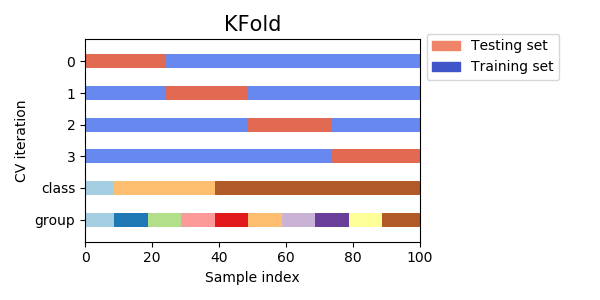
\includegraphics[width=1.0\columnwidth]{kfold2}
	\caption{Example of 4-Fold cross-validation}
	\label{fig:kfold}
\end{figure}

The example in Figure \ref{fig:kfold} represents a 4-Fold cross-validation execution. For each iteration the model is trained with a different partition of the dataset, and then the average of the three execution represents the performance of the model.

\subsubsection{Stratified KFold}

When the dataset's class are not equally balanced, it possible to have some folds without samples of a certain class. The stratification cross-validation ensures that each fold contains roughly the same proportions of classes of the entire dataset. Kohavi in \cite{kohavi1995study} states that normally stratification is better in terms of bias and variance, when compared to cross-validation.

\begin{figure}[!h]
	\centering
	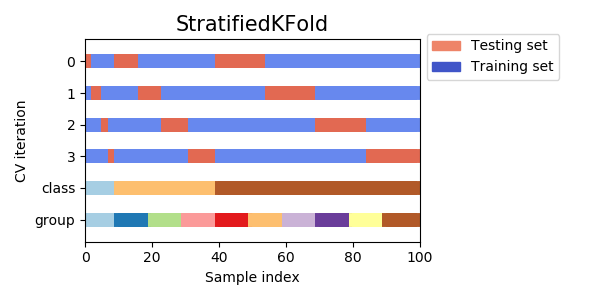
\includegraphics[width=1.0\columnwidth]{stratified}
	\caption{Example of stratified 4-Fold cross-validation}
	\label{fig:stratified}
\end{figure}

In Figure \ref{fig:stratified} is depicted an execution of stratified k-fold. As illustrated in the figure, a small portion of each class is taken as testing set at each fold.





\section{Features Selection}
\label{sec:feat_sel}
Features selection is a growing trend in machine learning problems. As technology advances, there is an increase in the quantity of data we can extract; this means bigger datasets to analyze and a decrease in performance and an increase in execution time. \\

Features selection is the process of selecting a subset of features that are more relevant for the model and ignore the rest.
The main goals of features selection are: \cite{guyon2003introduction}
\begin{itemize}
	\item Improve the performance of a classifier
	\item Reduce the time and cost of analysis
	\item Enhance data visualization and understanding
\end{itemize}

The idea behind feature selection is that if the dataset contains unnecessary or redundant features, those features can be removed without loss of information. \cite{bermingham2015application}

However, there is a distinction between usefulness and relevance of a feature, a set of useful features can exclude some redundant features, that could be, instead, relevant to the problem.\cite{kohavi1997wrappers} \textbf{da riverere da kohavi}

Features selection techniques can be grouped into three categories based on the approach used: \textbf{Filter methods}, \textbf{Wrapper methods}, \textbf{Embedded methods}.

\subsection{Filter methods}
Filter methods are applied directly to the dataset, so they are independent of the model used in the prediction. Compared to methods dependent on the model, such as wrapper or embedded methods, they have a better generalization of the problem, and they are faster. \cite{kohavi1997wrappers}

However, they have less predictive performance.  They rely only on the characteristics of the features in the training set and can show the relationship between variables. \cite{sanchez2007filter}
Usually, the filter methods rely on variable ranking. Ranking functions assign a score to each variable, and then the analyst can set a threshold of features to keep. 

Hastie et al. \cite{hastie2009elements} state that filter methods may be preferable at first to other features selection techniques because they are computationally and statistically scalable.  Computationally efficient because we only need to apply a function to n features in the dataset and statistically because they introduce bias, but they could have substantially less variance.

Scikit provides different functions for filter feature selection, such as Mutual information, chi-square, f-classification, variance threshold. Those methods are explained in detail in the next chapter.

\begin{figure}[!h]
	\centering
	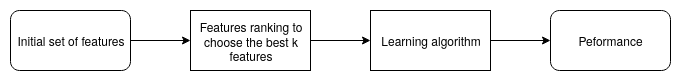
\includegraphics[width=1.0\columnwidth]{filter}
	\caption{Filter method flow}
	\label{fig:filter}
\end{figure}


\subsection{Wrapper methods}
\label{sec:wrapper}
Wrapper methods depend on the predictive model to choose a subset of features. The wrapper algorithm does not know the machine learning model used, and it is considered a black box \cite{kohavi1997wrappers}. 

The algorithm relies on the model to evaluate the performance of each subset of features. Each subset trains a model, and the model error rate establishes the score of the given subset. This procedure is repeated until an optimal subset of features is found. 

The main drawbacks of this method are that it is very computationally expensive, Amaldi et al. \cite{amaldi1998approximability} state that it is an NP-hard problem, and it can lead to overfitting if there are not enough data. Nevertheless, it usually gives the best result in predictive performance for the given model. \\

Efficient search algorithms are crucial to reducing the computational cost and time, and they are not always a synonym of decreasing in predictive performance. Greedy search algorithms are optimal for wrapper methods, and they are divided into two main categories: \textit{forward selection} and \textit{backward elimination}. \cite{reunanen2003overfitting}.

In \textit{forward selection}, the algorithm starts from an empty set, and at each iteration, it adds a new feature to the dataset. Instead, in \textit{backward elimination}, the algorithm starts from the whole dataset, and it removes a feature at each iteration, until it finds the best subset.

\begin{figure}[!h]
	\centering
	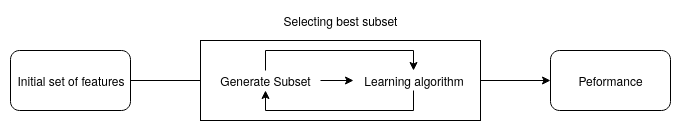
\includegraphics[width=1.0\columnwidth]{wrapper}
	\caption{Wrapper method flow}
	\label{fig:wrapper}
\end{figure}



\subsection{Embedded methods}

Embedded methods are a combination of the other two. They perform feature selection during the training process. \cite{guyon2003introduction} This technique allows the algorithms to be more efficient than wrapper methods. First of all, they do not need to split the dataset into training and testing sets. Secondly, they are faster because they do avoid to retrain the model for every subset of features.
The most common methods are \textit{Lasso} and \textit{Ridge regression} and \textit{decision tree}.

\textit{Lasso} and \textit{Ridge regression} penalize the beta coefficient by a factor, to avoid that the model focuses on a particular set of features.

\textit{Decision tree }algorithms select a feature at each recursive step, during the tree growing process, dividing the sample into smaller subsets. The more child node a tree has of the same class, the more important are the features.

\begin{figure}[!h]
	\centering
	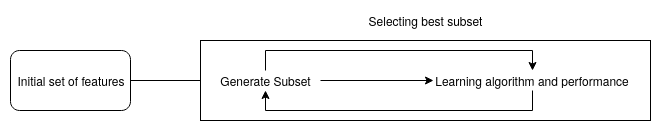
\includegraphics[width=1.0\columnwidth]{embedded}
	\caption{Embedded method flow}
	\label{fig:embedded}
\end{figure}